Dit verslag kijkt ook naar of verschillende omgevingsfactoren een effect hebben op het herkennen van kleuren. Zo zou de grootte van de omgeving de herkenning kunnen verbeteren of verslechteren, meer omgeving betekent namelijk dat de camera meer omgevingslicht binnenkrijgt. Alsook het licht kan een beïnvloedende factor zijn, de foto's behandelen twee soorten lichtinval: geen en artificieel licht. Buitenlicht zal niet besproken worden, de {\it Screen Caster} gaat ervan uit dat de schermen binnenshuis staan. Laatste omgevingsfactor is de helderheid van het scherm zelf. Heeft dit een grote invloed op de detectie? En hebben verschillende factoren een invloed op elkaar?

\subsubsection{Omgeving}
De foto's hebben verschillende groottes van omgeving. De omgeving kan groot ($\approx 80\%$), gemiddeld ($\approx 40\%$), klein ($\approx 10\%$) of niet aanwezig zijn. In figuur \ref{fig:omgeving}(a) zijn de bevindingen weergegeven. Per grootte van omgeving staat er weergegeven hoeveel procent van elke kleur juist werd gedetecteerd.

De detectie van kleuren gebeurd het beste bij een gemiddelde of kleine omgevingsgrootte. Wanneer de omgeving groot is, scoort de herkenning het slechtst. In figuur \ref{fig:omgeving}(b) staat per kleur welke kleur foutief is herkent, enkel en alleen bij een grote omgeving. Wat opvalt is dat vooral zwart als foute kleur naar voor komt en dan vooral bij groen, wit en geel. Dit is toe te wijzen aan het feit dat met meer lichtinval de schermen donkerder tonen op de foto. Door een grotere omgeving zal de artificiële inteligentie in de camera de focus niet meer op het scherm leggen. Als zwart niet meer nodig is en de restrictie op de lichtheid bij HSL niet meer geldt, kan dit probleem opgelost zijn, dit vergt echter verder onderzoek.
\begin{figure}
	\begin{subfigure}{0.5\textwidth}
	\centering
	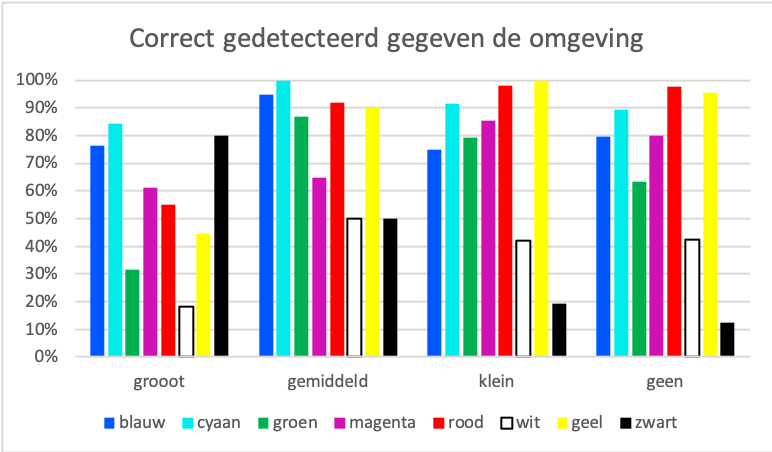
\includegraphics[scale=0.6]{img/Environment}
	\caption{Per kleur correct gedetecteerd met gegeven omgevingsgrootte.}
	\end{subfigure}
	\begin{subfigure}{0.5\textwidth}
	\centering
	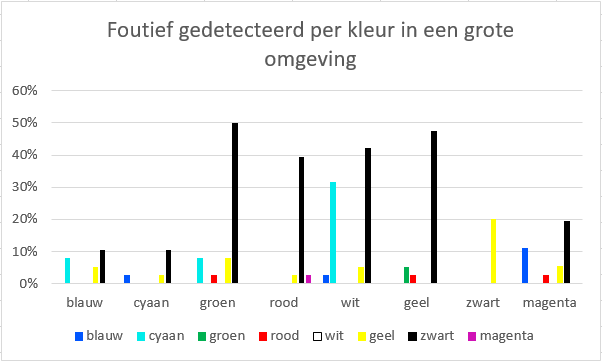
\includegraphics[scale=0.6]{img/BigEnvPerColor}
	\caption{Per kleur de foutief herkende kleur in grote omgeving.}
	\end{subfigure}
	\caption{Grafieken met betrekking tot de omgevingsgrootte.}
	\label{fig:omgeving}
\end{figure}

\subsubsection{Lichtinval}
Dit verslag behandelt twee soorten lichtinval, artificieel en helemaal geen lichtinval. In figuren \ref{fig:lichtinval}(a) en \ref{fig:lichtinval}(b) staan de gedetecteerde kleuren per kleur bij respectievelijk artificieel en geen lichtinval. Rood komt bij artificieel licht in elke kleur voor, dit is toe te wijzen aan het licht dat een rode schijn achterlaat op de schermen. Zonder achtergrondverlichting  komt vooral zwart terug foutief terug. Dit is te wijten aan het algoritme dat naast het scherm gedetecteerd heeft.

Zwart detecteren is opvallend slecht bij artificieel licht, door de strenge herkenning ($L < 10$) en reflectie is deze niet herkent bij artificieel licht. Geel en cyaan komen veel voor bij detectie van wit, ook hier is de strenge herkenning ($L > 90$) de oorzaak.

\begin{figure}
	\begin{subfigure}{0.5\textwidth}
	\centering
	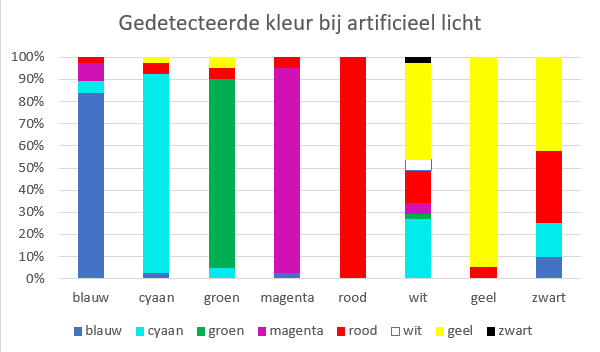
\includegraphics[scale=0.6]{img/artificialLightning}
	\caption{Artificieel lichtinval.}
	\end{subfigure}
	\begin{subfigure}{0.5\textwidth}
	\centering
	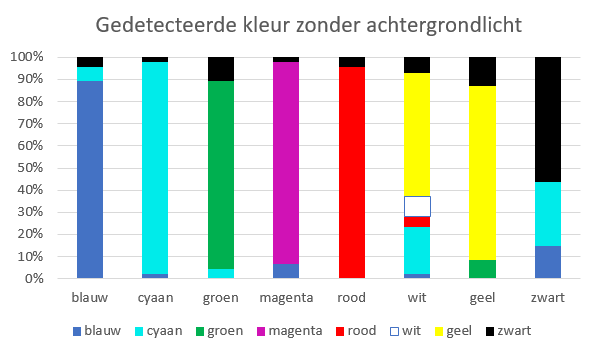
\includegraphics[scale=0.6]{img/noneLightning}
	\caption{Zonder lichtinval.}
	\end{subfigure}
	\caption{Gedetecteerde kleur per kleur. (HSL)}
	\label{fig:lichtinval}
\end{figure}

\subsubsection{Helderheid scherm}
In figuur \ref{fig:helderheid} staat het aantal procent correct gedetecteerde kleur per helderheid van het scherm. De laagste helderheid scoort het slechts, kleuren zijn donkerder en minder goed zichtbaar. Bij de drie andere helderheden is geen groot verschil op te merken. De schermhelderheid heeft geen grote invloed op de detectie van de schermen.
\begin{figure}
	\centering
	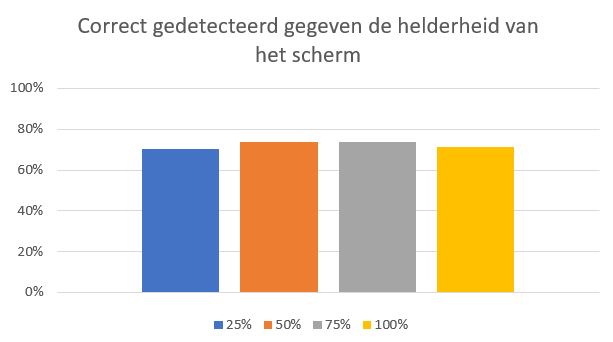
\includegraphics[scale=0.7]{img/brightness}
	\caption{Procent juist gedetecteerde kleur per kleur met gegeven schermhelderheid. (HSL)}
	\label{fig:helderheid}
\end{figure}
